\lesson{}{Optimization}

\newpage
% \label{sub_sec:diffeq}

\subsubsection{Introduction}
Although colloquially used in everyday language, optimization (or commonly spelled by the intelligentsia as \textit{optimisation}) has a rich and deep philosophical meaning in mathematics and physics. The entire field can arguably be considered the core idea of any dynamical system that seeks equilibrium. In physics and chemistry, these dynamical systems seek paths that will reduce its energy state to some equilibrium point. Similar problems in finance, engineering, operations research, and/or parameter \textit{learning} can also be cast following the same metaphor by maximizing or minimizing a desired quantity by varying the \textit{decision variables} (also referred to as \textit{optimization variables} or \textit{manipulated variables}). In some applications, the system is driven to a certain state following a local descent path to the nearest minimum energy state, as does a ball rolling down a hill to find peace in a valley. Other examples of optimization appear out of randomness, such as life in Darwin's game of survival of the fittest. 

In general, we can approximate these problem statements mathematically as a set of inputs $\boldsymbol{x} \in \mathcal{X}$ and outputs $\boldsymbol{y} \in \mathcal{Y}$, via some mapping of the form $f \ : \ \mathcal{R}^n \rightarrow \mathcal{R}$. For mathematical optimization, the goal is to find some input $\boldsymbol{x} \in \mathcal{R}^n$ that minimizes or maximizes the output $y \in \mathcal{R}$. The canonical, or standard form of such an \textit{optimisation} problem can be read as the following: 

\begin{align*}
    \min_{\boldsymbol{x}} \quad & f_0(\boldsymbol{x}) \\
    \text{subject to} \quad & f_i(\boldsymbol{x}) \leq b_i, \quad i = 1, ..., m. 
\end{align*}

which reads as ``minimize $f_0(\boldsymbol{x})$ subject to $f_i(\boldsymbol{x}) \leq b_i$ for all $i = 1, ..., m$", where $f_0(x)$ is the objective function $f_0 \ : \ \mathcal{R}^n \rightarrow \mathcal{R}$ (also referred to as the cost or evaluation function), the vector $\boldsymbol{x} \in \mathcal{R}^n$, the functions $f_i \ : \ \mathcal{R}^n \rightarrow \mathcal{R}, \ i = 1, ..., m$ are the inequality \textit{constraints}, and the constants $b_1, \ ..., b_m$ are the bounds for the constraints. We call the best choice $\boldsymbol{x}^\ast$ the \textit{optimal solution}. For more details on notation, see Boyd. 

As one might expect, it is only natural for individuals pursuing the topic of \textit{optimisation} to cleverly conclude (hopefully prior to beginning graduate school, and god forbid, before middle life) that \textit{``oh my god, everything is an optimisation problem"}, thus leading the individual to rich and deep thoughts of the nature of reality, philosophy, and an optimal utopia. But alas, remember the words of Steven Boyd echoing through the hallowed convex halls of Stanford University, ''to say everything is an optimisation problem is a stupid tautology". In fact, it does not mean anything to shout such a revelation as nothing can be concluded from such a whimsical statement. What matters is what the \textit{optimisation} problem is, since most optimisation problems \textit{you can not solve}. So oh dear reader, come to this clever conclusion as rapidly as possible, and the wipe your shoes of such dirt before entering mathematical wonders of \textit{optimisation}. 

But oh, what \textit{optimisation} problems can we solve, our dear reader (who may or may not exist) must be wondering. Here, I seek to describe just that. Let us first consider the set of all tractable \textit{optimisation} problems $\min_{\boldsymbol{x}} \ f_0(\boldsymbol{x})$. The tractability of such a problem first begins with the the structure of $f_0(\boldsymbol{x})$. Under some circumstances, $f_0(x)$ is an explicit function in which we can analyze or operate on. For example, the univariate objective function $f_0(\boldsymbol{x}) = (x + 2)^2 + 1$ is a familiar one from basic maths courses from early secondary school. The minimization of such a function is as easy whipping out our $\frac{d}{dx}$ operator, setting its derivative equal to zero, and solving for $x$. In this simplified case, the solution to the \textit{optimisation} problem is written as $x^\ast = -2$. In this case, the \textit{optimisation} problem is considered to have an \textit{analytical solution}. And thus we have our first approach to solving an \textit{optimisation} problem. Unfortunately, analytical solutions are far from achievable for most tractable problems. \textit{Numerical solutions} shall be our toolset for solving the nastier \textit{optimisation} problems. It is in this realm we seek to develop and compare algorithms for solving a tractable $\min_{x} \ f_0(\boldsymbol{x})$. 

The following sections will describe numerical techniques for solving tractable optimization problems. These problems can generally be subdivided into two categories: convex optimization and non-convex (blackbox) optimization. 

\subsubsection{Gradient-based methods}

\noindent {\it {\bf Newton's method}}:

Let us first consider an convex objective $f_0(x)$ and method in which we can approach solving the minimization. Convexity enables us to makes certain assumptions about optimality conditions. One optimality condition being 

\begin{equation*}
    \nabla_{\boldsymbol{x}} f_0(\boldsymbol{x}) = 0,
\end{equation*}

or more simply, we would like to find the root of the gradient of $f_0(\boldsymbol{x})$.

Newton's method is a simple numerical approach used for find roots of an equation if an initial candidate solution is close the exact solution. Here I derive Newton's method using a Taylor Series expansion. 

Suppose $f_0(\boldsymbol{x})$ is a continuous function on a closed interval $[a, b]$ and has $n+1$ continuous derivatives on the open interval $(a, b)$. If $x, c \in (a, b)$, then the expansion of $f_0(x)$ about c is:

\begin{equation*}
    f(c) + f'(c)(x - c) + \frac{1}{2!} f''(c)(x-c)^2 + \frac{1}{3!} f'''(c)(x-c)^3 + ... + \frac{1}{n!}f^n(c)(x-c)^n
\end{equation*}

or more concisely:

\begin{equation*}
    f(x) \approx \sum^{\infty}_{k=0} \frac{1}{k!} f^{(k)}(c)(x-c)^k
\end{equation*}

Provided an initial guess value $\boldsymbol{x}^j$,

By approximating $f_0(\boldsymbol{x})$ using this expansion, we can find the optimal $x^\ast$ by expanding $\nabla_x f_0(x)$ around a initial guess value $x^j$, which at optimum should be equal to zero:

\begin{equation*}
    \nabla_x f_0(x^{j+1}) = \nabla_x f_0(x^{j}) + \nabla_x(\nabla_x f_0(x^j))(x^{j+1} - x^{j}) + \mathcal{O}(x^{j+1}-x^{j})^2 = 0|_{x^{j+1} = x^\ast}. 
\end{equation*}

The resulting error $\mathcal{O}(x^{j+1}-x^{j})^2$ indicates that this optimization method is a second-order gradient-based approach. Rearranging the above equation yields:

\begin{equation*}
    - \nabla_x f_0(x^j) = \nabla_x(\nabla_x f_0(x^j))(x^{j+1} - x^{i})
\end{equation*}

where we seek to solve for $x^{j+1}$, where $\nabla_x(\nabla_x f_0(x^j))$ is the Hessian. If $x$ is a vector, than a matrix inversion is required to solve for $x^{j+1}$. 

\begin{equation*}
    \boldsymbol{x}^{j+1} = \boldsymbol{x}^j - [\nabla_x(\nabla_x f_0(\boldsymbol{x}^j)]^{-1} \nabla_x f_0(\boldsymbol{x}^j).
\end{equation*}

Explicitly, the Hessian is defined as:

\begin{equation*}
    H = \nabla_x(\nabla_x f_0(\boldsymbol{x}_i)) = 
    \begin{bmatrix}
        \frac{\partial f_0^2}{\partial x_1^2} & \frac{\partial f_0^2}{\partial x_1 \partial x_2} & \ldots & \frac{\partial f_0^2}{\partial x_1 \partial x_n} \\
        \frac{\partial f_0^2}{\partial x_2 \partial x_1} & \frac{\partial f_0^2}{\partial x_2^2} & \ldots & \frac{\partial f_0^2}{\partial x_2 \partial x_n} \\
        \vdots & \vdots & \ddots & \vdots \\
        \frac{\partial f_0^2}{\partial x_n \partial x_1} & \ldots & \ldots & \frac{\partial f_0^2}{\partial x_n^2}
    \end{bmatrix}
\end{equation*}

This means that use of Newton's methods for gradient descent requires an inversion of a $n\times n$ matrix to compute the next candidate solution. The update equation can be explicitly referred to as:

\begin{equation*}
    \begin{bmatrix}
        x_1^{j+1} \\
        \vdots \\
        x_n^{j+1}
    \end{bmatrix} = 
    \begin{bmatrix}
        x_1^{j} \\
        \vdots \\
        x_n^{j}
    \end{bmatrix} - 
    \begin{bmatrix}
        \frac{\partial f_0^2}{\partial x_1^2} & \ldots & \frac{\partial f_0^2}{\partial x_1 \partial x_n} \\
        \vdots & \ddots & \vdots \\
        \frac{\partial f_0^2}{\partial x_n \partial x_1} & \ldots & \frac{\partial f_0^2}{\partial x_n^2}
    \end{bmatrix}
    \begin{bmatrix}
        \frac{\partial f_0}{\partial x_1} \\
        \vdots \\
        \frac{\partial f_0}{\partial x_n}
    \end{bmatrix}. 
\end{equation*}

Sometime, we do not have an explicit form of $f_0(\boldsymbol{x})$ and therefore do not have access to the gradients directly. We can approximate these gradients numerically (see Section on Numerical Methods), however Newton's method quickly deteriorates as a viable option as $n \rightarrow \infty$ since matrix inversion has computational complexity on the order of $\mathcal{O}(n^3)$. 

\noindent {\it {\bf First-order methods} }



Gradient descent optimizes a function by using first-order gradient information, while Newton's method optimizes a function utilizing second-order gradient information. The most basic implementation of gradient descent computes the gradient of the objective function and slightly perturbs the current position. Although first-order methods are considerably faster, these algorithms can be unstable and perform poorly on non-convex functions. Consider the example in which parameters of a model are being tuned to fit a data set:

\begin{tcolorbox}[colback=green!5!white,colframe=green!75!black]
Let $\theta$ be the parameters for a function approximator $f_0(x)$. Gradient descent can computed iteratively as 

\begin{equation*}
    \theta^{i+1} = \theta^i - \gamma \nabla_\theta f_0(x), \quad x \in \mathcal{D}
\end{equation*}

where $\gamma$ is a hyper parameter chosen to determine the incremental step size performed by optimizer.

\end{tcolorbox}

\begin{tcolorbox}[colback=gray!5!white,colframe=gray!75!black]
 An example implementation in Python is shown below while attempting to optimize the non-convex \href{https://en.wikipedia.org/wiki/Test_functions_for_optimization}{Beale Function}:

 \begin{minted}{python}
 # manual gradients and hessians for each funciton
def grad_beale(curr_loc, ord=1, method=1):
    """ computes gradient and hessian
        inputs:
            - {x, y} coords: ndarray
            - ord: 1 or 2 for gradient or hessian
            - method: 1 or 2 for analtyical or numerical
        outputs: 
            - gradient
            - hessian """
    x = curr_loc[0]
    y = curr_loc[1]

    # compute gradient
    dfdx = 2 * (1.5 - x + x * y) * (-1 + y) + \
           2 * (2.25 - x + x * y ** 2) * (-1 + y ** 2) + \
           2 * (2.6250 - x + x * y ** 3) * (-1 + y ** 3)
    dfdy = 2 * (1.5 - x + x * y) * x + \
           2 * (2.25 - x + x * y ** 2) * (2 * x * y) + \
           2 * (2.6250 - x + x * y **3) * (3 * x * y ** 2)

    gradient = np.array([dfdx, dfdy])
    
    if ord == 1:
        return gradient
    
    elif ord == 2:
        # compute hessian
        ddfddx = 2 * (y - 1) * (y - 1) + \
                2 * (y * y - 1) * (y * y - 1) + \
                2 * (y * y * y - 1) * (y * y * y - 1)
        ddfdydx = 4 * x * (y ** 2 - 1) + \
                  4 * y * (x * y * y - x + 2.25) + \
                  6 * x * (y * y * y - 1) * y * y + \
                  y * y ** 2 * (x * y * y * y - x + 2.625) + \
                  2 * x * (y - 1) + \
                  2 * (x * y - x + 1.5)
        ddfddy = 18 * x * x * y * y * y * y + \
                8 * x * x * y * y + \
                4 * x * (x * y * y - x + 2.25)

        hessian = np.array([[ddfddx, ddfdydx], [ddfdydx, ddfddy]])
        return gradient, hessian

 \end{minted}
\end{tcolorbox}

\begin{tcolorbox}[colback=gray!5!white,colframe=gray!75!black]
\begin{minted}{python}
def grad_descent(grad_fn, init_loc=[0, 0], n_steps=10000, f=None):
gamma = 1e-6

# initialize trajectories
traj = np.zeros((n_steps, len(init_loc)))
traj[0, :] = np.array(init_loc)

for i in range(1, n_steps):
    if f is not None:
        traj[i, :] = traj[i - 1, :] \
                   - gamma * grad_fn(f=f, 
                                     curr_loc=traj[i - 1, :], 
                                     ord=1)
    else:
        traj[i, :] = traj[i - 1, :] \
                   - gamma * grad_fn(traj[i - 1, :], 
                                     ord=1)

return traj

for i in range(len(initial_points)):
trajectories_gd = grad_descent(grad_beale, initial_points[i])
output, fig, ax = beale([], [])
ax.scatter(trajectories_gd[:-1, 0], trajectories_gd[:-1, 1], 
           s=25, facecolor='orange')
ax.scatter(trajectories_gd[-1, 0], trajectories_gd[-1, 1], 
           s=150, facecolor='m', marker='*', label='gd opt')
\end{minted}
\end{tcolorbox}

\begin{figure}[H]
    \centering
    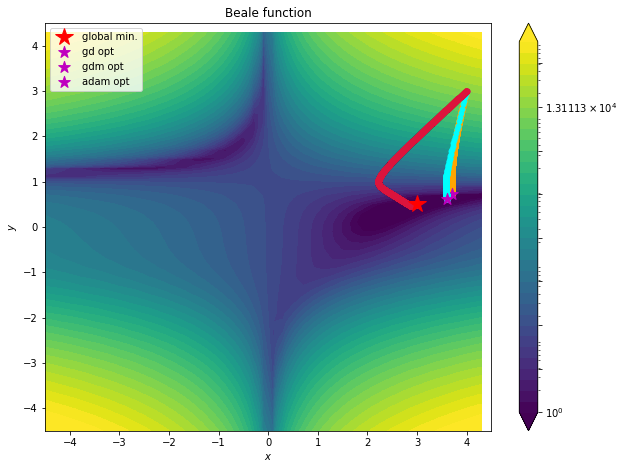
\includegraphics[width = 15cm]{figures/gd_beale.png}
    \caption{A benchmark comparison between gradient descent, gradient descent + momentum, and ADAptive Momentum (ADAM) gradient descent on the non-convex Beale Function}
    \label{fig:learning_dist}
\end{figure}


\subsubsection{Blackbox optimization + non-gradient-based methods}

\textit{Genetic algorithms}
\textit{Simulated annealing}
\textit{Bayesian optimization}



\begin{question}
\label{q:1}
Let's say you are trying to learn from a distribution of data. What do you do?

\refA{sol:1}
\end{question}

\begin{solution}
\label{sol:1}
You simply apply RL until you achieve an h-index of 130. 

\refQ{q:1}
\end{solution}



\newpage